\documentclass[letterpaper, 10 pt, conference]{ieeeconf}

\IEEEoverridecommandlockouts                              
\overrideIEEEmargins
% See the \addtolength command later in the file to balance the column lengths
% on the last page of the document

\usepackage{hyperref}

% The following packages can be found on http:\\www.ctan.org
%\usepackage{graphics} % for pdf, bitmapped graphics files
%\usepackage{epsfig} % for postscript graphics files
%\usepackage{mathptmx} % assumes new font selection scheme installed
%\usepackage{times} % assumes new font selection scheme installed
%\usepackage{amsmath} % assumes amsmath package installed
%\usepackage{amssymb}  % assumes amsmath package installed

\title{\LARGE \bf
Summer Documentation 
}


\author{Saikat Mondal 
\thanks{ Thanks to all the seniors and 2nd years for their help}
}


\begin{document}



\maketitle 
\thispagestyle{empty}
\pagestyle{empty}


%%%%%%%%%%%%%%%%%%%%%%%%%%%%%%%%%%%%%%%%%%%%%%%%%%%%%%%%%%%%%%%%%%%%%%%%%%%%%%%%
\begin{abstract}
%\textbf{Should be half column long. Should be clear enough to explain your whole documentation. Similar to a TL;DR}

In the last summer I mainly worked for The International Aerial Robotics competition mission 7 which will be held this year.
Mission 7 will challenge teams to demonstrate 
three  new  behaviors  that  have  never  been  attempted in any of the past six IARC missions.\\
First,
Interaction    between    Aerial    Robots    and    
Ground  Robots:\\


1.   A  square  arena  will be marked  on  the  ground 
in an indoor GPS-free arena.  This square 
arena will be 20 meters on each side.  The 
boundary  shall  consist  of  wide  white  lines  
bounding the sides of the square arena, with 
a wide red line on one end, and a wide green 
line on the other end as shown in the figure.
Page 7 of  24\\

2.   Ten  (10)  iRobot  Create  programmable autonomous
ground  robots of color red and green  will  be  placed  at  the  center  of the arena.  The orientation of the ground 
robots  will  be  such  that  they  will  initially  
move  in  all  directions  of  the  arena.    The 
aerial robot will launch from a white side of 
the arena.\\

3.   When the run begins, the ground robots begin 
to  move  toward  the  boundaries  of  the  arena,  
but  as  collisions  occur,  they  will  reorient  
themselves  to  move  in  different  directions  
or,  after  about  20  seconds  of  travel,  they  
will redirect themselves.  Eventually when a 
ground  robot  reaches  any  edge  of  the  square  
arena,  it  is  permanently  removed  from  the  
arena.\\

4.   Each robot has a tactile switch on the top.  
If  an  aerial  robot  comes  close  enough  to  
just “touch the top” of the ground robot, the 
ground  robot  will  change  its  direction  of  
movement by 45 degrees (clockwise).\\

5.   It  is  the  job  of  the  autonomous  aerial 
robot  to  redirect  the  ground  robots  and  
herd  them  toward  the  green  side  of  the  
arena such that as many as possible cross 
over the green line.  This is achieved by 
descending onto the top of a ground robot, 
the  effect  of  which  will  be  to  cause  the  
ground  robot  to  change  its  direction  by  
45  degrees  (clockwise).    For  example, 
descending  upon  the  same  ground  robot  
twice  will  result  in  the  robot’s  direction  
changing 90 degrees (clockwise).  Landing 
in  front  of  a  ground  robot  to  induce  a  
collision which will also cause the robot to 
change its direction of movement, but by 
180 degrees.  Ground robots that happen 
to  collide  will  likewise  change  direction  
by 180 degrees.\\

6.   In  addition  to  the  10  ground  robots  that 
need  to  be  herded  toward  the  green  end  
of  the  arena,  there  will  be  4  robots  with  
tall   cylinders   extending   vertically   from   
their  upper  surface    (up  to  two  meters  
maximum).    These  special  ground  robots 
will be preprogrammed to circle within the 
arena and to serve two functions.  The first 
function is as a source to help randomize 
the motion of the other 10 target robots by 
periodically causing collisions that reorient 
those  robots.    The  second  function  is  to 
provide moving vertical obstacles that must 
be avoided by the aerial robot as it uses its 
sense and avoid technologies.  Should more 
than  two  impacts  occur  between  the  aerial  
robot  and  one  of  the  cylindrical  obstacles,  
the run will be terminated.\\

7.   The autonomous aerial robot must analyze 
the  directions  of  the  various  ground  robots  
and  redirect  them  toward  the  green  end  of  
the  arena  while  avoiding  the  four  obstacle  
robots.  Aerial robots must stay within the 
boundaries of the arena, but are allowed to 
go up to approximately two meters outside 
the  boundary  momentarily  (for  up  to  5  
seconds).  Aerial robots must not exceed an 
altitude of three meters above the floor, and 
they are allowed to land inside the arena.  \\

8.   Strategies  involved  would  be  to  redirect 
robots  that  are  closer  to  the  red  or  white  
edges  of  the  arena  before  contending  with  
robots that are either still close to the center 
of the arena, or which are generally on track 
toward the green end of the arena.\\

9.   All  of  the  robots  are  autonomous  (both 
ground and air).  When the run begins, the 
aerial robot should do everything that it can 
get  the  ground  robots  to  the  green  edge  of  
the arena while avoiding the obstacle robots.  
The run will be over when all of the ground 
robots  either  reach  the  green  edge  of  the  
arena,  or  go  out  of  bounds  on  either  of  the  
white edges or the red edge.  In any event, 
assuming  that  there  are  still  active  (non  
obstacle) ground robots in the arena, the run 
will be terminated after 10 minutes, and any Page 9 of  24
robots  not  yet  over  the  green  line  will  be  
considered  to  have  gone  out  of  bounds  for  
the purposes of scoring.  Completing a run 
in  less  time  is  a  determining  factor  in  the  
selection of the final grand prize winner.\\

10. To diminish the effects of bad “luck,” each 
team  will  be  allowed  to  perform  a  total  of  
three  times,  and  the  one  best  performance  
out of the three attempts will be used as the 
final score for that team.  The team with the 
highest score at the end of Mission 7a will 
be declared the winner.\\

11.   Mission 7a design strategies and capabilities 
will   include   speed,   energy   endurance,   
object    recognition,    air    vehicle/ground    
vehicle interaction, tracking moving targets, 
maneuvering to land (momentarily) on (or in 
front of) a moving target, target identification, 
target  prioritization,  knowledge  of  the 
progress of ALL targets, obstacle avoidance, 
and the ability to navigate without external 
cues such as GPS or beacons.  All of these 
must be demonstrated during Mission 7a in 
order to be eligible for Mission 7b.\\
\end{abstract}




%%%%%%%%%%%%%%%%%%%%%%%%%%%%%%%%%%%%%%%%%%%%%%%%%%%%%%%%%%%%%%%%%%%%%%%%%%%%%%%%
\section{INTRODUCTION}

I was the autonomous ground bots of both Green and Red colors in both the front and bottom camera which will be attached with the drone.

\section{Problem Statement}
\textbf{ My Problem Statement was to detect the autonomous ground bots using the video feeds given by the bottom camera.}

 Now for bottom camera it wasn't tough enough but the main problem was with the front camera. Because there the parts out side grid was also visible.

\section{INITIAL ATTEMPTS}

Initially I thought to dectect moving objects on ground and then detect their color.But the ground bots were too slow compared to our drone. So this approach could not be used.

\section{Related Work}

Then I thought to use Hough Circle detection as the ground bots were of round shape.But here the problem was that those will be looked as circle only if we see from top. So in case of front camera those seemed to be ellipse.so this method can not be used for front camera.\\

So then I thought to use histogram back projection method.

\textbf{ Histogram Back Projection : }
\\
 \textbf{1. Histogram }
An histogram a spectrum of intensity repartition. Concretely this is a list that contains for each possible value of pixel the number of pixels that have this value. You can say well, but in the end how can it be really useful ? for which purposes ? For instance calculate the histogram of an area on a photography, then the same area on another photography from another point of view for instance is more likely to have the same histogram. Indeed OpenCV provide all the needed function to do it. thank’s to \textbf{CalcHist} and \textbf{ CompareHist} that return a float of the distance (accuracy). \\

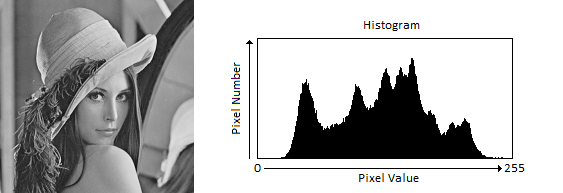
\includegraphics [scale =0.55 ] {lennaWithHist.png}

An image with it's histogram (right side)\\

\textbf{2. Histogram Back Projection}

The backprojection is calculated from the histogram. It basically replace every pixel by it’s probability to occur in the image.\\


1.    Back Projection is a way of recording how well the pixels of a given image fit the distribution of pixels in a histogram model.\\
2.    To make it simpler: For Back Projection, you calculate the histogram model of a feature and then use it to find this feature in an image.\\
3.    Application example: If you have a histogram of flesh color (say, a Hue-Saturation histogram ), then you can use it to find flesh color areas in an image:\\

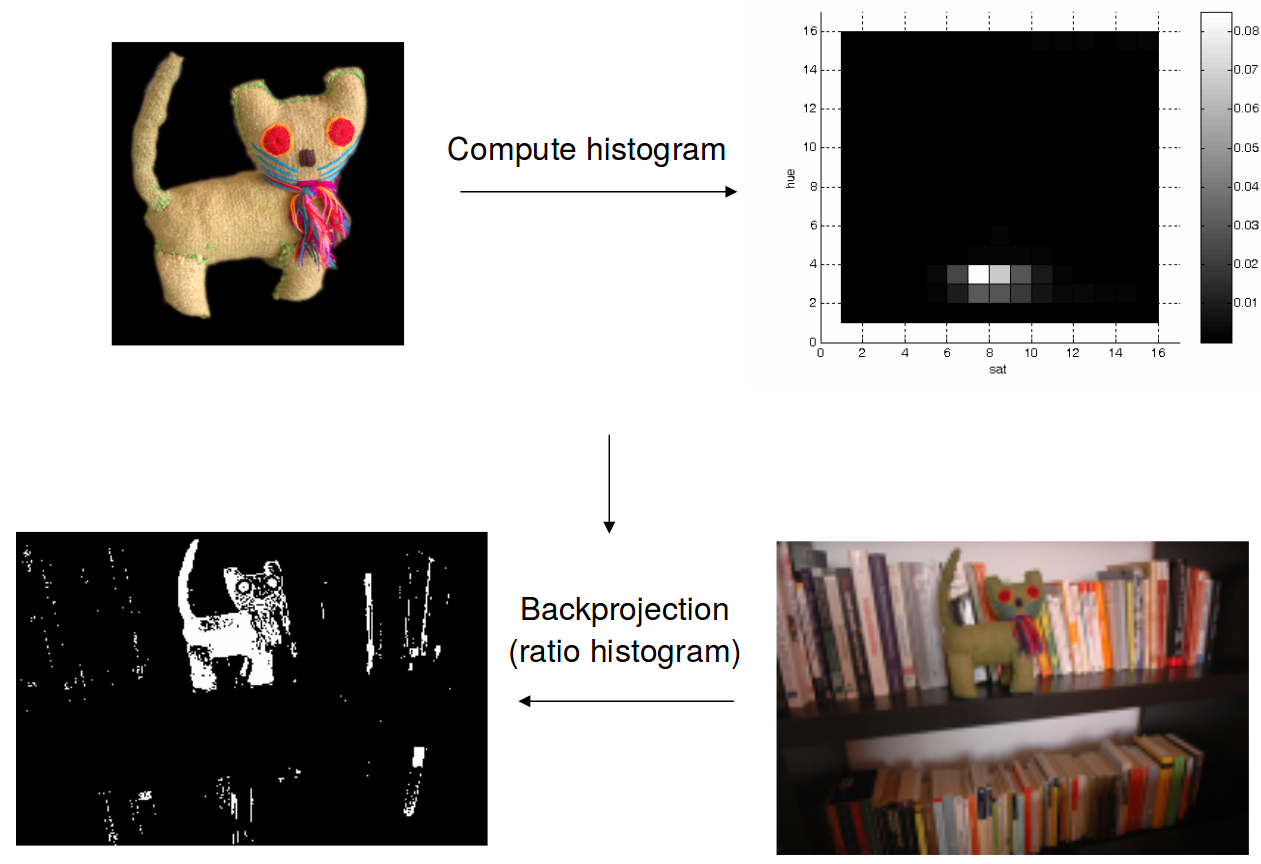
\includegraphics [ scale =0.20] {histBackeg.png}

\textbf{ My approach :}\\

1. First I compute the ratio histogram using the opencv devide function\\
2.Then perform back projection using the opencv calcBackProject function\\

I have pushed my programmes in github.And here are the links\\
link 1 :
\href{https://github.com/Saikat2019/IARC\_onlyImgProc/blob/master/botDetect\_histBack.cpp}{botDetect\_histBack.cpp}\\
link 2 :
\href{https://github.com/Saikat2019/IARC\_onlyImgProc/blob/master/botDetect\_in\_video.cpp}{botDetect\_in\_video.cpp}

\textbf{result on bot }\\
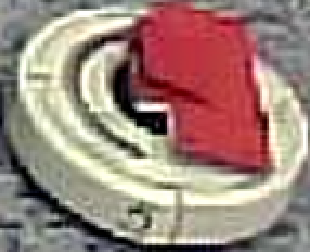
\includegraphics[scale =0.30]{model.png}\\
\textbf{model image of red bot}\\

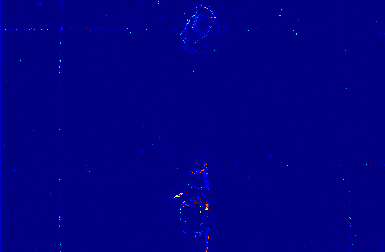
\includegraphics[scale =0.85 ]{backprojectonimage.png}\\
\textbf{ratio histogram backprojection to the image}\\

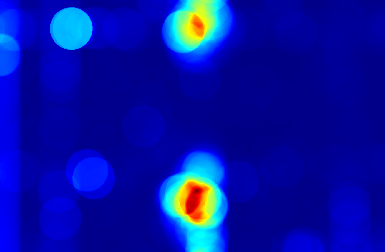
\includegraphics[scale =0.85 ]{convolutionwithcircularmask.png}\\
\textbf{convolution with circular mask}\\

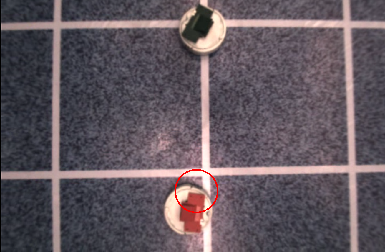
\includegraphics[scale = 0.85]{Detected.png}\\
\textbf{Detected position}

But the problem with this approach was when there was no ground bot in the video feed it was showing false detection.so we could not use this approach

\section{Final Approach}

\textbf{The circle Hough Transform (CHT) is a feature extraction technique for detecting circles.}\\
 It is a specialization of Hough Transform. The purpose of the technique is to find circles in imperfect image inputs. The circle candidates are produced by “voting” in the Hough parameter space and then select the local maxima in a so-called accumulator matrix. 
\textbf{Theory :}\\
In a two-dimensional space, a circle can be described by:\\
     ( x − a ) 2 + ( y − b ) 2 = r 2           \\

where (a,b) is the center of the circle, and r is the radius. If a 2D point (x,y) is fixed, then the parameters can be found according to (1). The parameter space would be three dimensional, (a, b, r). And all the parameters that satisfy (x, y) would lie on the surface of an inverted right-angled cone whose apex is at (x, y, 0). In the 3D space, the circle parameters can be identified by the intersection of many conic surfaces that are defined by points on the 2D circle. This process can be divided into two stages. The first stage is fixing radius then find the optimal center of circles in a 2D parameter space. The second stage is to find the optimal radius in a one dimensional parameter space. \\

now we can get the value of the radius of the ground bot in pixels from the calculated height and camera matrix.\\

\textbf{Find parameters with known radius R :}

If the radius is fixed, then the parameter space would be reduced to 2D (the position of the circle center). For each point (x, y) on the original circle, it can define a circle centered at (x, y) with radius R according to (1). The intersection point of all such circles in the parameter space would be corresponding to the center point of the original circle. 
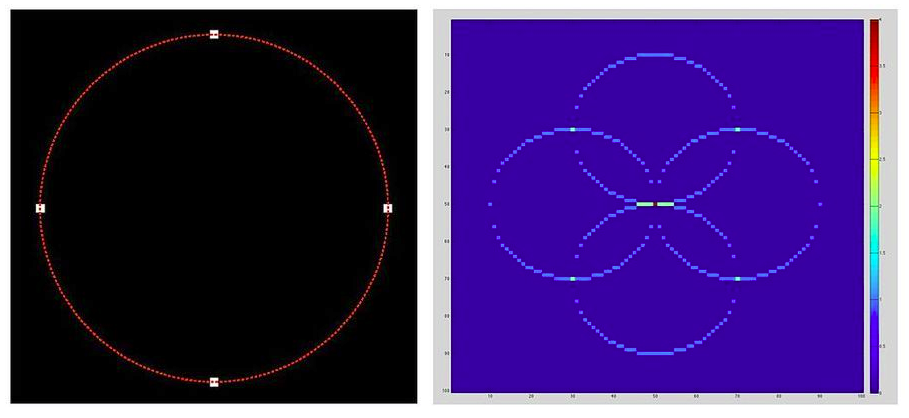
\includegraphics [scale =0.27]{houghCir1.png}
Consider 4 points on a circle in the original image (left). The circle Hough transform is shown in the right. Note that the radius is assumed to be known. For each (x,y) of the four points (white points) in the original image, it can define a circle in the Hough parameter space centered at (x, y) with radius r. An accumulator matrix is used for tracking the intersection point. In the parameter space, the voting number of points through which the circle passing would be increased by one. Then the local maxima point (the red point in the center in the right figure) can be found. The position (a, b) of the maxima would be the center of the original circle. 

\textbf{Voting :}\\
In practice, an accumulator matrix is introduced to find the intersection point in the parameter space. First, we need to divide the parameter space into “buckets” using a grid and produce an accumulator matrix according to the grid. The element in the accumulator matrix denotes the number of “circles” in the parameter space that passing through the corresponding grid cell in the parameter space. The number is also called “voting number”. Initially, every element in the matrix is zeros. Then for each “edge” point in the original space, we can formulate a circle in the parameter space and increase the voting number of the grid cell which the circle passing through. This process is called “voting”.\\

After voting, we can find local maxima in the accumulator matrix. The positions of the local maxima are corresponding to the circle centers in the original space. \\

But this hough circle tranform could not be applied for front camera, because from there the ground bots will be viewed as ellipse.\\

so for front camera video feed we used thresholding and blob detection to to detect the ground bots.\\

but here the problem was that sometimes we may get the view out side the grid so then an area may be detected as a ground bot outside the grid.\\

so first we need to subtract the areas out side grid from the video.so for this we first tried trigonometry to get the real coordinates of each pixels using the current coordinates and angle of the front camera.\\

link to the code in github :\\
\href{https://github.com/Saikat2019/IARC\_onlyImgProc/blob/master/gridSubt2.cpp}{grid subtract}\\

but this was giving wrong output. so we tried to use camera matrix and solvePNP function to get the real cordinates.\\
link to the code :\\
\href{https://github.com/Saikat2019/IARC_onlyImgProc/blob/master/wtp2.cpp}{world to pixel}\\
But this was also giving out put with some error.

So then we tried to use HSV thresholding to remove the grid from the feed.
So,after this we will left with the area out side grid(if any).And then if we take intersection we will get the view inside the grid only.\\

link to the code in github :\\
\href{https://github.com/Saikat2019/IARC_onlyImgProc/blob/master/GridSubtFinal.cpp}{HSV thresholding}

\begin{thebibliography}{99} 
\bibitem{c1}\href{https://en.wikipedia.org/wiki/Circle_Hough_Transform}{wikipedia} 
\bibitem{c2}\href{https://docs.opencv.org/3.4/d4/d70/tutorial_hough_circle.html}{opencv hough circle transform} 
\bibitem{c3}\href{http://www.lira.dist.unige.it/teaching/SINA_08-09/slides-prev/sina-image-processing-point.pdf}{Histogram Backprojection}
\bibitem{c4}\href{https://docs.opencv.org/2.4/doc/tutorials/imgproc/histograms/back_projection/back_projection.html}{OpenCV Histogram Backprojection}
\end{thebibliography}

\end{document}
